\section{Tổng quan mô hình và pipeline của hệ thống}

Pipeline tổng quát của hệ thống gồm các bước chính. Đầu tiên, dữ liệu thô được đọc từ file CSV và xử lý ở bước preprocessing. Trong bước này, các token và nhãn BIO trong dataset được chuyển thành danh sách ground truth entities để phục vụ đánh giá. Tiếp theo, hệ thống sử dụng regex-based detector để nhận diện các thực thể có cấu trúc rõ ràng như email, số điện thoại và URL. Sau đó, context-based detector được dùng để nhận diện các thực thể phụ thuộc nhiều vào ngữ cảnh như tên người, tổ chức, địa điểm,địa chỉ và username. Kết quả từ hai detector được đưa vào module merger để gộp, loại bỏ trùng lặp và xử lý các entity bị chồng lấn. Cuối cùng, hệ thống thực hiện ẩn danh văn bản và đánh giá kết quả bằng các chỉ số Precision, Recall và F1-score.

\begin{figure}[H]
    \centering
    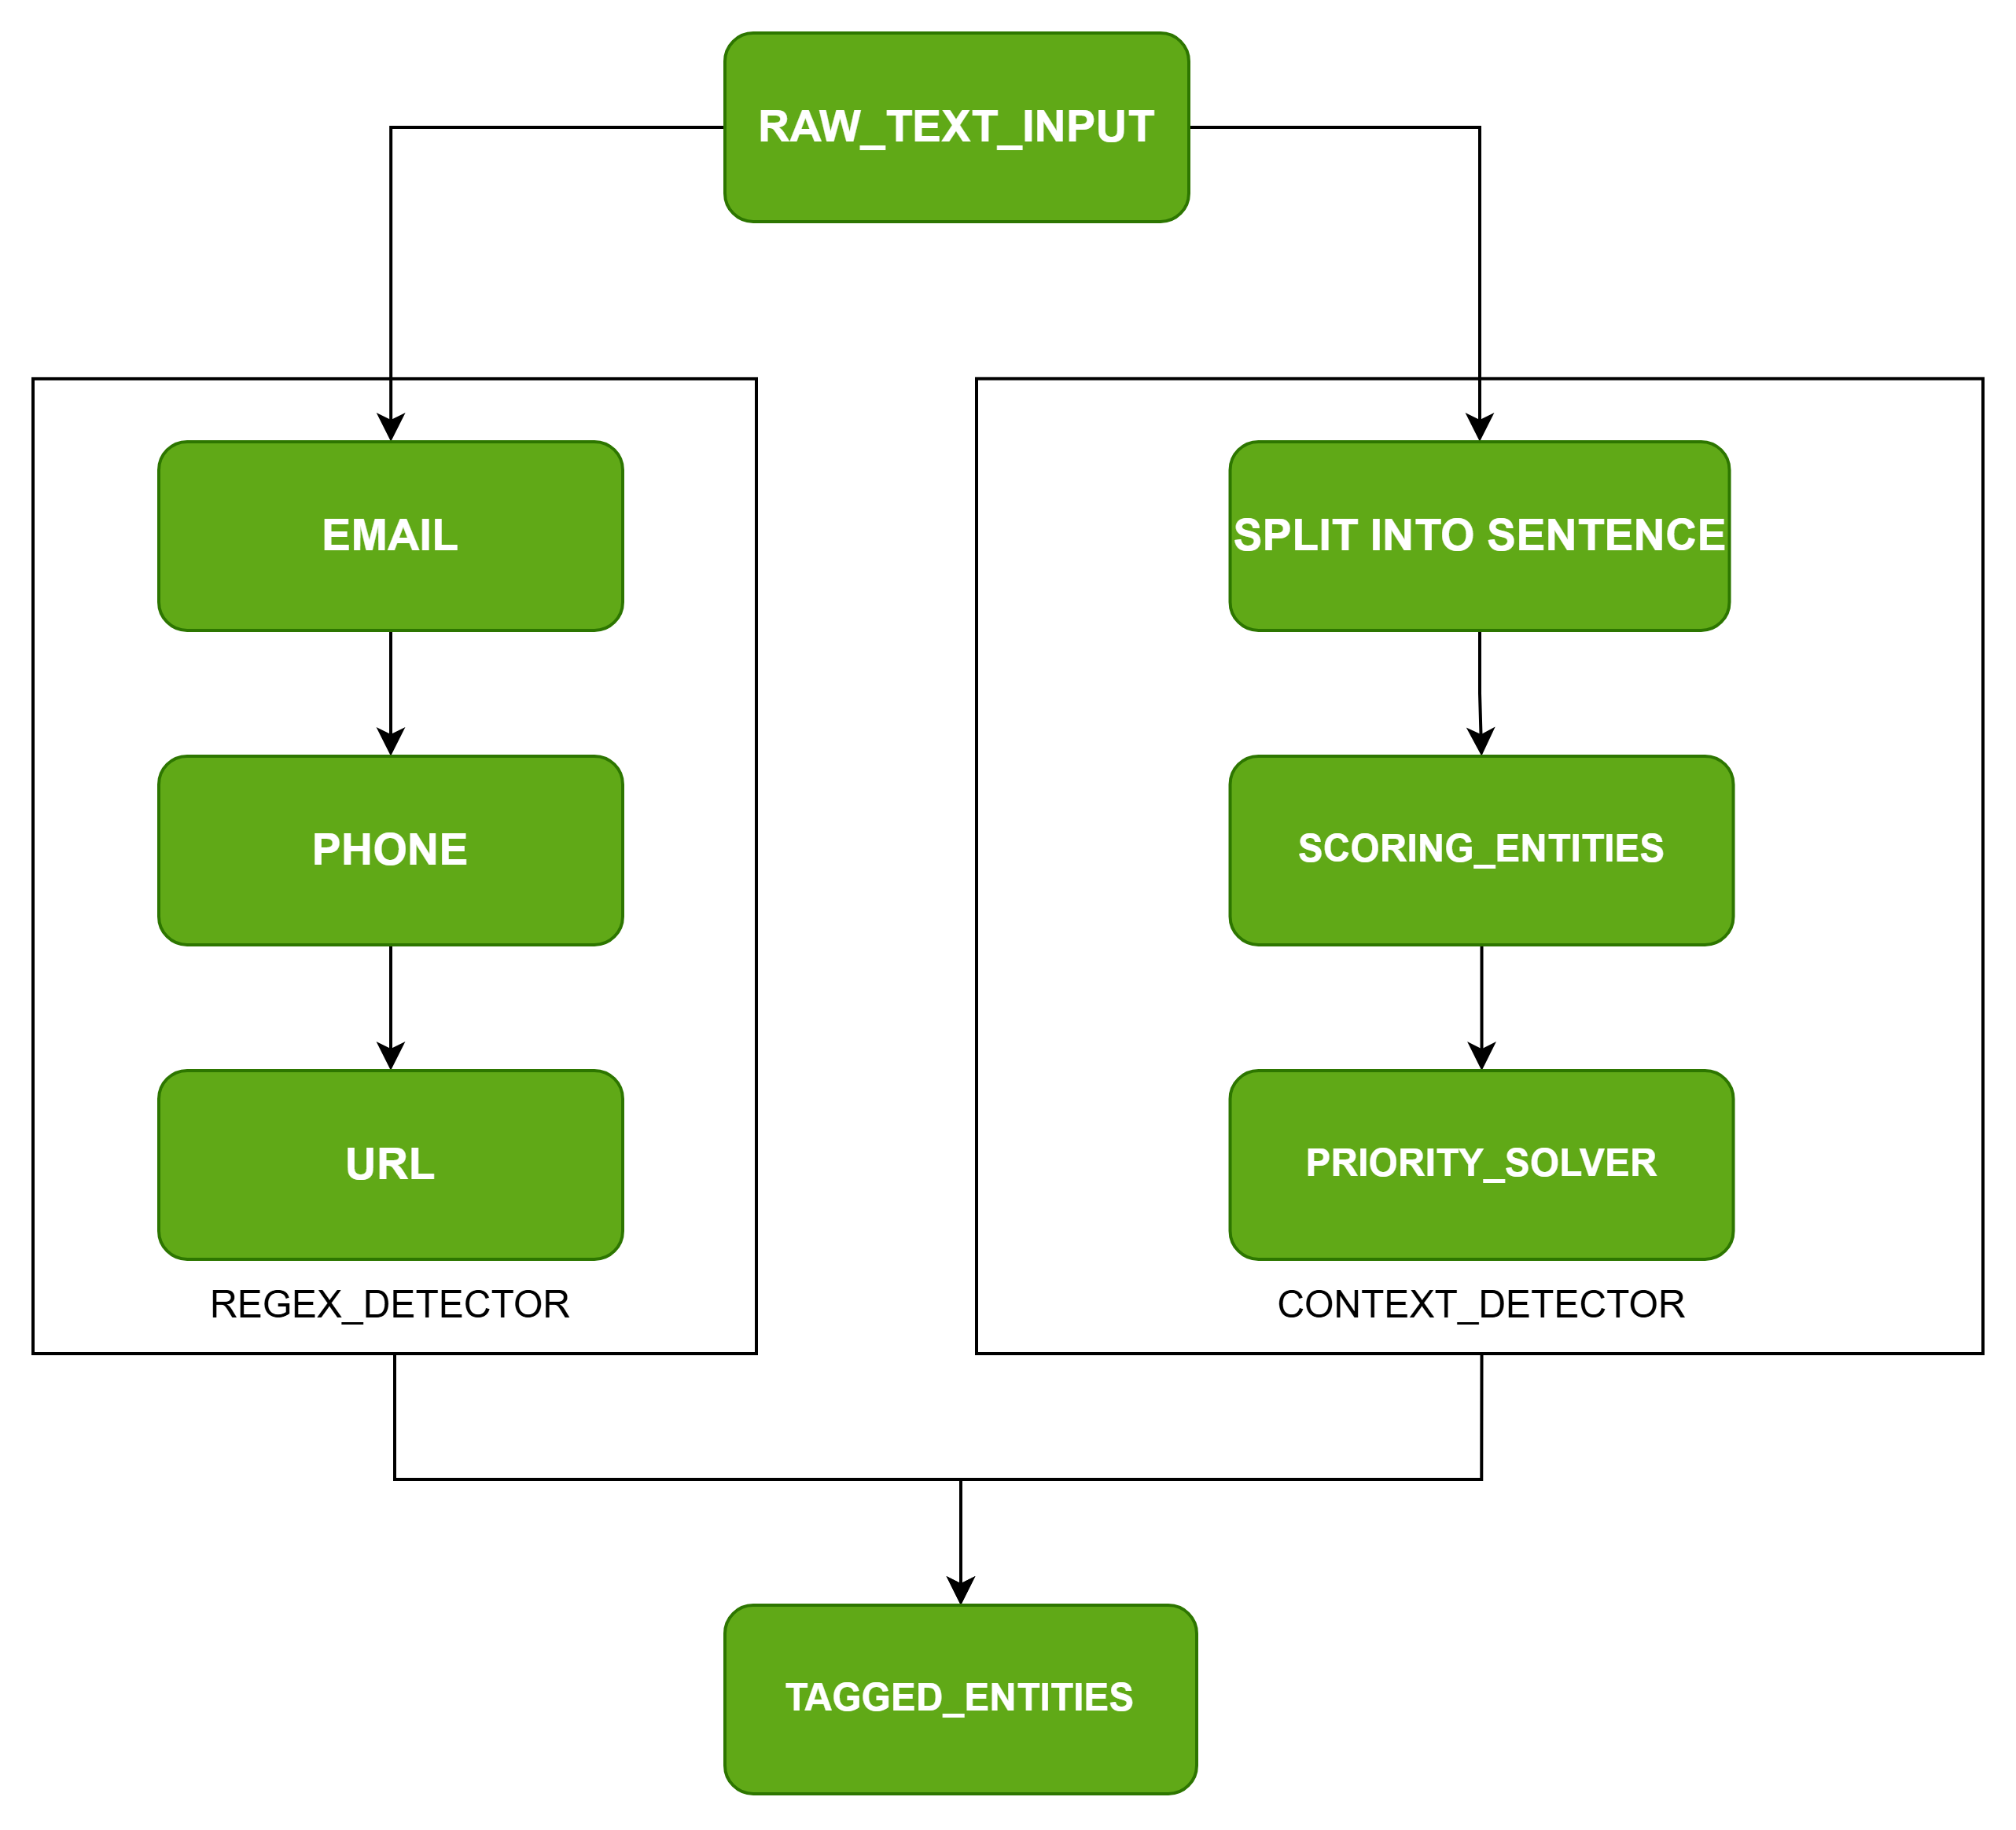
\includegraphics[width=0.7\textwidth]{graphics/PIPELINE.png}
    \caption{Pipeline tổng quát của hệ thống}
\end{figure}